\documentclass[11pt,a4paper]{report}

% ============================================================
% PACKAGES
% ============================================================
\usepackage[utf8]{inputenc}
\usepackage[T1]{fontenc}
\usepackage{lmodern}
\usepackage[margin=1in]{geometry}
\usepackage{graphicx}
\usepackage{xcolor}
\usepackage{hyperref}
\usepackage{booktabs}
\usepackage{longtable}
\usepackage{array}
\usepackage{tabularx}
\usepackage{enumitem}
\usepackage{fancyhdr}
\usepackage{titlesec}
\usepackage{tcolorbox}
\usepackage{tikz}
\usepackage{multicol}
\usepackage{multirow}
\usepackage{pifont}
\usepackage{fontawesome5}
\usepackage{mdframed}
\usepackage{etoolbox}
\usepackage{calc}
\usepackage{lipsum}

% ============================================================
% COLOR DEFINITIONS
% ============================================================
\definecolor{primaryblue}{RGB}{25, 55, 95}
\definecolor{accentblue}{RGB}{52, 152, 219}
\definecolor{darkgray}{RGB}{45, 52, 54}
\definecolor{lightgray}{RGB}{245, 246, 250}
\definecolor{successgreen}{RGB}{39, 174, 96}
\definecolor{warningorange}{RGB}{243, 156, 18}
\definecolor{phase1color}{RGB}{155, 89, 182}
\definecolor{phase2color}{RGB}{52, 152, 219}
\definecolor{phase3color}{RGB}{46, 204, 113}

% ============================================================
% HYPERREF CONFIGURATION
% ============================================================
\hypersetup{
    colorlinks=true,
    linkcolor=primaryblue,
    filecolor=accentblue,
    urlcolor=accentblue,
    citecolor=primaryblue,
    pdftitle={Comprehensive Curriculum: Prompt Engineering and LLM Application Development},
    pdfauthor={},
    pdfsubject={Prompt Engineering Curriculum},
    pdfkeywords={prompt engineering, LLM, AI, machine learning, curriculum}
}

% ============================================================
% PAGE STYLE CONFIGURATION
% ============================================================
\pagestyle{fancy}
\fancyhf{}
\fancyhead[L]{\small\textcolor{darkgray}{\leftmark}}
\fancyhead[R]{\small\textcolor{darkgray}{Prompt Engineering Curriculum}}
\fancyfoot[C]{\thepage}
\renewcommand{\headrulewidth}{0.4pt}
\renewcommand{\footrulewidth}{0pt}

% ============================================================
% TITLE FORMATTING
% ============================================================
\titleformat{\chapter}[display]
{\normalfont\huge\bfseries\color{primaryblue}}
{\chaptertitlename\ \thechapter}{20pt}{\Huge}

\titleformat{\section}
{\normalfont\Large\bfseries\color{primaryblue}}
{\thesection}{1em}{}

\titleformat{\subsection}
{\normalfont\large\bfseries\color{darkgray}}
{\thesubsection}{1em}{}

\titleformat{\subsubsection}
{\normalfont\normalsize\bfseries\color{darkgray}}
{\thesubsubsection}{1em}{}

% ============================================================
% CUSTOM ENVIRONMENTS
% ============================================================
\newtcolorbox{learningobjectives}{
    colback=lightgray,
    colframe=accentblue,
    fonttitle=\bfseries,
    title={\faIcon{bullseye} Learning Objectives},
    arc=3mm,
    boxrule=1pt
}

\newtcolorbox{keyconcepts}{
    colback=lightgray,
    colframe=successgreen,
    fonttitle=\bfseries,
    title={\faIcon{lightbulb} Key Concepts},
    arc=3mm,
    boxrule=1pt
}

\newtcolorbox{practicalexercise}{
    colback=lightgray,
    colframe=warningorange,
    fonttitle=\bfseries,
    title={\faIcon{laptop-code} Practical Exercise},
    arc=3mm,
    boxrule=1pt
}

\newtcolorbox{resourcebox}{
    colback=lightgray,
    colframe=phase1color,
    fonttitle=\bfseries,
    title={\faIcon{book} Resources},
    arc=3mm,
    boxrule=1pt
}

\newtcolorbox{assessmentbox}{
    colback=lightgray,
    colframe=primaryblue,
    fonttitle=\bfseries,
    title={\faIcon{clipboard-check} Assessment Criteria},
    arc=3mm,
    boxrule=1pt
}

\newtcolorbox{timebox}{
    colback=lightgray,
    colframe=darkgray,
    fonttitle=\bfseries,
    title={\faIcon{clock} Estimated Time},
    arc=3mm,
    boxrule=1pt
}

\newtcolorbox{deliverablebox}{
    colback=lightgray,
    colframe=successgreen,
    fonttitle=\bfseries,
    title={\faIcon{flag-checkered} Deliverable},
    arc=3mm,
    boxrule=1pt
}

% ============================================================
% DOCUMENT BEGIN
% ============================================================
\begin{document}

% ============================================================
% TITLE PAGE
% ============================================================
\begin{titlepage}
\begin{center}

\vspace*{1cm}


\begin{tikzpicture}
\fill[primaryblue] (0,0) rectangle (16,2);
\node[white, font=\Huge\bfseries] at (8,1) {COMPREHENSIVE CURRICULUM};
\end{tikzpicture}

\vspace{1.5cm}

{\Huge\bfseries\textcolor{primaryblue}{Prompt Engineering \&\\[0.3cm] LLM Application Development}}

\vspace{1cm}


\begin{tikzpicture}
\draw[accentblue, line width=2pt] (0,0) -- (10,0);
\end{tikzpicture}

\vspace{1cm}

{\Large\textcolor{darkgray}{A Structured Learning Path from\\Fundamentals to Production-Ready AI Systems}}

\vspace{2cm}

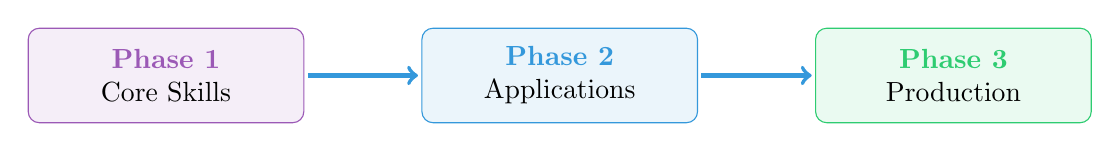
\begin{tikzpicture}
\node[draw=phase1color, fill=phase1color!10, rounded corners, minimum width=3.5cm, minimum height=1.2cm, align=center] at (0,0) {\textbf{\textcolor{phase1color}{Phase 1}}\\Core Skills};
\node[draw=phase2color, fill=phase2color!10, rounded corners, minimum width=3.5cm, minimum height=1.2cm, align=center] at (5,0) {\textbf{\textcolor{phase2color}{Phase 2}}\\Applications};
\node[draw=phase3color, fill=phase3color!10, rounded corners, minimum width=3.5cm, minimum height=1.2cm, align=center] at (10,0) {\textbf{\textcolor{phase3color}{Phase 3}}\\Production};
\draw[->, line width=1.5pt, accentblue] (1.8,0) -- (3.2,0);
\draw[->, line width=1.5pt, accentblue] (6.8,0) -- (8.2,0);
\end{tikzpicture}

\vspace{2cm}

{\large Duration: 12--16 Weeks}

\vspace{0.5cm}

{\large Target Audience: Software Engineers \& Developers}

\vfill


\begin{tikzpicture}
\fill[lightgray] (0,0) rectangle (16,1.5);
\node[darkgray, font=\small] at (8,0.75) {Version 1.0 | \today};
\end{tikzpicture}

\end{center}
\end{titlepage}

% ============================================================
% TABLE OF CONTENTS
% ============================================================
\tableofcontents
\newpage

% ============================================================
% CHAPTER: EXECUTIVE SUMMARY
% ============================================================
\chapter{Executive Summary}

\section{Course Overview}

This comprehensive curriculum provides a structured pathway for software engineers to master prompt engineering and build production-ready applications powered by Large Language Models (LLMs). The program is designed around three progressive phases that build upon each other, taking learners from fundamental prompting techniques through application development to full-stack AI engineering practices.

The curriculum synthesizes knowledge from the most authoritative resources in the field, including seminal texts such as \textit{Prompt Engineering for Generative AI}, \textit{AI Engineering: Building Applications with Foundation Models}, and the \textit{LLM Engineer's Handbook}, complemented by continuously updated documentation from leading AI providers including OpenAI, Anthropic, and Google.

\section{Target Audience}

This curriculum is designed for:
\begin{itemize}[leftmargin=1.5cm]
    \item \textbf{Software Engineers} seeking to integrate LLM capabilities into applications
    \item \textbf{Backend/Full-Stack Developers} building AI-powered products
    \item \textbf{Technical Product Managers} requiring deep understanding of LLM systems
    \item \textbf{ML Engineers} transitioning to LLM-focused roles
    \item \textbf{Technical Writers and Content Creators} working with generative AI
\end{itemize}

\section{Prerequisites}

\begin{tabularx}{\textwidth}{lX}
\toprule
\textbf{Category} & \textbf{Requirements} \\
\midrule
Programming & Proficiency in Python (intermediate level); familiarity with REST APIs \\
Development & Basic understanding of version control (Git); experience with package managers \\
Concepts & Fundamental understanding of machine learning concepts (helpful but not required) \\
Tools & Access to OpenAI API, Anthropic API, or similar LLM providers \\
Mindset & Willingness to experiment iteratively and embrace empirical approaches \\
\bottomrule
\end{tabularx}

\section{Program Structure}

\begin{center}
\begin{tabularx}{0.95\textwidth}{>{\centering\arraybackslash}p{2.5cm} >{\centering\arraybackslash}p{2cm} X >{\centering\arraybackslash}p{2.5cm}}
\toprule
\textbf{Phase} & \textbf{Duration} & \textbf{Focus Area} & \textbf{Outcome} \\
\midrule
\textcolor{phase1color}{\textbf{Phase 1}} & 2--4 weeks & Core prompting skills, patterns, and evaluation & Personal prompt cookbook \\
\textcolor{phase2color}{\textbf{Phase 2}} & 4--6 weeks & Building LLM-powered applications and agents & 2--3 portfolio projects \\
\textcolor{phase3color}{\textbf{Phase 3}} & 4--6 weeks & Production systems, MLOps, and engineering practices & Production playbook \\
\bottomrule
\end{tabularx}
\end{center}

\section{Learning Outcomes}

Upon successful completion of this curriculum, learners will be able to:

\begin{enumerate}[leftmargin=1.5cm]
    \item Design and implement effective prompts across text, code, and multimodal applications
    \item Apply systematic prompt patterns including chain-of-thought, few-shot learning, and critique-and-revise
    \item Build functional LLM applications incorporating retrieval-augmented generation (RAG)
    \item Implement tool use and function calling within LLM systems
    \item Evaluate prompt and system quality using appropriate metrics and methodologies
    \item Deploy LLM applications with proper monitoring, feedback loops, and cost management
    \item Make informed architectural decisions between prompting, fine-tuning, and RAG approaches
    \item Navigate the trade-offs between different model providers and deployment strategies
\end{enumerate}

% ============================================================
% CHAPTER: PHASE 1 - CORE PROMPTING SKILLS
% ============================================================
\chapter{Phase 1: Core Prompting Skills}
\label{ch:phase1}

\begin{timebox}
\textbf{Duration:} 2--4 weeks \\
\textbf{Study Hours:} 20--40 hours total \\
\textbf{Recommended Pace:} 8--12 hours per week
\end{timebox}

\vspace{0.5cm}

\begin{learningobjectives}
By the end of Phase 1, learners will:
\begin{itemize}
    \item Reliably obtain high-quality outputs from GPT, Claude, Gemini, and similar models
    \item Apply 20--30 distinct prompting patterns with confidence
    \item Understand the principles underlying effective prompt construction
    \item Evaluate and iteratively improve prompt performance
    \item Construct prompts for text, code, and image generation tasks
\end{itemize}
\end{learningobjectives}

% --------------------------------------------------------
\section{Module 1.1: Foundations of Prompt Engineering}
% --------------------------------------------------------

\subsection{Overview}

This foundational module establishes the theoretical and practical groundwork for all subsequent learning. Students will develop an intuitive understanding of how language models process and respond to prompts, along with the fundamental techniques that form the basis of effective prompting.

\begin{keyconcepts}
\begin{itemize}
    \item How LLMs process text and generate responses (tokenization, attention, sampling)
    \item The prompt-completion paradigm and its implications
    \item Zero-shot vs. few-shot prompting fundamentals
    \item The role of context windows and token limits
    \item Temperature, top-p, and other generation parameters
\end{itemize}
\end{keyconcepts}

\subsection{Reading Assignments}

\begin{resourcebox}
\textbf{Primary Reading:}
\begin{enumerate}
    \item \textit{The Art of Prompt Engineering with ChatGPT} -- Chapters 1--3 (Core Techniques)
    \item OpenAI Prompt Engineering Guide -- Complete reading
    \item Anthropic Prompt Engineering Documentation -- Overview and Best Practices sections
\end{enumerate}

\textbf{Supplementary Reading:}
\begin{enumerate}
    \item DAIR.AI Prompt Engineering Guide -- Introduction section
    \item Google Cloud Prompt Engineering Guide -- Fundamentals
\end{enumerate}
\end{resourcebox}

\subsection{Topics Covered}

\subsubsection{Understanding Language Model Behavior}

Students will explore the fundamental mechanisms that govern how language models interpret and respond to prompts:

\begin{itemize}[leftmargin=1.5cm]
    \item \textbf{Tokenization:} How text is converted to tokens and why token boundaries matter for prompt design
    \item \textbf{Context Windows:} Working within token limits; strategies for context management
    \item \textbf{Probabilistic Generation:} Understanding that outputs are sampled from probability distributions
    \item \textbf{Instruction Following:} How models are trained to follow instructions (RLHF, Constitutional AI)
    \item \textbf{Model Capabilities and Limitations:} Realistic expectations for different model sizes and types
\end{itemize}

\subsubsection{Core Prompting Techniques}

\begin{longtable}{p{4cm}p{10cm}}
\toprule
\textbf{Technique} & \textbf{Description and Application} \\
\midrule
\endhead
Role Prompting & Assigning a persona or expert role to the model (e.g., ``You are a senior software architect...'') to influence response style and depth \\
\midrule
Instruction Clarity & Writing unambiguous, specific instructions; avoiding vague language; being explicit about format and scope \\
\midrule
Constraint Specification & Defining boundaries, length limits, style requirements, and output formats \\
\midrule
Context Setting & Providing relevant background information; establishing scope; defining terminology \\
\midrule
Output Formatting & Specifying JSON, XML, Markdown, or custom formats; using delimiters and structure \\
\midrule
Positive/Negative Constraints & Explicitly stating what to include and what to avoid \\
\midrule
Task Decomposition & Breaking complex requests into clear, sequential steps \\
\bottomrule
\end{longtable}

\subsection{Practical Exercises}

\begin{practicalexercise}
\textbf{Exercise 1.1.1: Vague to Precise Transformation}

Take the following vague prompts and transform them into precise, well-structured prompts. Document your reasoning for each transformation.

\begin{enumerate}
    \item ``Write something about climate change''
    \item ``Help me with my code''
    \item ``Explain machine learning''
    \item ``Write a marketing email''
\end{enumerate}

\textbf{Deliverable:} For each prompt, provide the improved version and a 2--3 sentence explanation of the changes made and why.
\end{practicalexercise}

\begin{practicalexercise}
\textbf{Exercise 1.1.2: Role Prompting Comparison}

Select a technical topic you're familiar with. Write three versions of a prompt asking for an explanation:
\begin{enumerate}
    \item No role specified
    \item Role: ``You are a college professor''
    \item Role: ``You are an experienced practitioner teaching a junior colleague''
\end{enumerate}

Compare the outputs systematically: tone, depth, examples used, accessibility.

\textbf{Deliverable:} Written analysis (500--700 words) comparing the outputs and identifying when each role framing would be most appropriate.
\end{practicalexercise}

\begin{practicalexercise}
\textbf{Exercise 1.1.3: Generation Parameter Exploration}

Using the same prompt, generate outputs with different temperature settings (0.0, 0.5, 0.7, 1.0) and document the differences. Repeat with different top-p values.

\textbf{Deliverable:} Table of results with observations about creativity vs. consistency trade-offs.
\end{practicalexercise}

% --------------------------------------------------------
\section{Module 1.2: Advanced Prompting Patterns}
% --------------------------------------------------------

\subsection{Overview}

Building on foundational techniques, this module introduces sophisticated patterns that enable more complex reasoning and higher-quality outputs from language models.

\begin{keyconcepts}
\begin{itemize}
    \item Chain-of-thought (CoT) prompting and its variants
    \item Few-shot learning and example selection strategies
    \item Self-consistency and ensemble approaches
    \item Critique-and-revise patterns
    \item Tree-of-thought and advanced reasoning structures
    \item Prompt chaining and decomposition
\end{itemize}
\end{keyconcepts}

\subsection{Reading Assignments}

\begin{resourcebox}
\textbf{Primary Reading:}
\begin{enumerate}
    \item \textit{Prompt Engineering for Generative AI} -- Chapters on Five Principles of Prompting
    \item \textit{Prompt Engineering for Generative AI} -- Chapters on evaluation and multi-modal prompts
    \item DAIR.AI Guide -- Chain-of-Thought Prompting section
\end{enumerate}

\textbf{Supplementary Reading:}
\begin{enumerate}
    \item Original CoT paper: ``Chain-of-Thought Prompting Elicits Reasoning in Large Language Models''
    \item ``Self-Consistency Improves Chain of Thought Reasoning in Language Models''
\end{enumerate}
\end{resourcebox}

\subsection{Topics Covered}

\subsubsection{Chain-of-Thought Prompting}

Chain-of-thought (CoT) prompting represents one of the most significant advances in prompt engineering, enabling language models to solve complex reasoning problems by explicitly generating intermediate steps.

\begin{longtable}{p{4cm}p{10cm}}
\toprule
\textbf{CoT Variant} & \textbf{Description} \\
\midrule
\endhead
Zero-shot CoT & Adding ``Let's think step by step'' or similar phrases to trigger reasoning without examples \\
\midrule
Few-shot CoT & Providing examples that demonstrate the reasoning process \\
\midrule
Self-consistency & Generating multiple reasoning paths and selecting the most consistent answer \\
\midrule
Tree-of-Thought & Exploring multiple reasoning branches and evaluating them \\
\midrule
Program-aided CoT & Using code execution to verify or assist reasoning steps \\
\bottomrule
\end{longtable}

\subsubsection{Few-Shot Learning Strategies}

\begin{itemize}[leftmargin=1.5cm]
    \item \textbf{Example Selection:} Choosing diverse, representative examples; avoiding bias
    \item \textbf{Example Ordering:} Impact of example sequence on model performance
    \item \textbf{Example Format:} Structuring input-output pairs consistently
    \item \textbf{Negative Examples:} When and how to include counterexamples
    \item \textbf{Dynamic Few-Shot:} Selecting examples based on input similarity
\end{itemize}

\subsubsection{Iterative Refinement Patterns}

\begin{longtable}{p{4cm}p{10cm}}
\toprule
\textbf{Pattern} & \textbf{Application} \\
\midrule
\endhead
Critique-and-Revise & Model generates output, then critiques and improves it \\
\midrule
Multi-turn Refinement & Progressive improvement through conversation \\
\midrule
Self-Evaluation & Model assesses its own output against criteria \\
\midrule
Adversarial Prompting & Testing outputs for weaknesses and edge cases \\
\midrule
Constitutional AI Patterns & Applying principles-based evaluation and revision \\
\bottomrule
\end{longtable}

\subsection{Practical Exercises}

\begin{practicalexercise}
\textbf{Exercise 1.2.1: Chain-of-Thought Implementation}

Solve the following problem types using both zero-shot and few-shot CoT:
\begin{enumerate}
    \item Multi-step arithmetic word problems
    \item Logical reasoning puzzles
    \item Code debugging scenarios
    \item Strategic decision analysis
\end{enumerate}

Compare accuracy and reasoning quality between approaches.

\textbf{Deliverable:} Documented prompts and outputs with comparative analysis.
\end{practicalexercise}

\begin{practicalexercise}
\textbf{Exercise 1.2.2: Few-Shot Example Engineering}

Create a few-shot prompt for a text classification task (e.g., sentiment analysis, intent detection). Systematically vary:
\begin{enumerate}
    \item Number of examples (1, 3, 5, 10)
    \item Example diversity
    \item Example ordering
\end{enumerate}

\textbf{Deliverable:} Performance analysis across variations with recommendations.
\end{practicalexercise}

\begin{practicalexercise}
\textbf{Exercise 1.2.3: Critique-and-Revise Pipeline}

Build a three-stage prompt pipeline:
\begin{enumerate}
    \item Initial generation of a technical document (API documentation, tutorial, etc.)
    \item Self-critique against specified criteria (clarity, completeness, accuracy)
    \item Revision incorporating critique feedback
\end{enumerate}

\textbf{Deliverable:} Complete pipeline with prompts at each stage; before/after comparison.
\end{practicalexercise}

% --------------------------------------------------------
\section{Module 1.3: Prompt Evaluation and Quality Assurance}
% --------------------------------------------------------

\subsection{Overview}

Systematic evaluation is critical for developing reliable prompts. This module covers methodologies for assessing prompt quality, establishing baselines, and implementing continuous improvement processes.

\begin{keyconcepts}
\begin{itemize}
    \item Evaluation metrics for different task types
    \item Creating golden test sets
    \item A/B testing prompts
    \item Automated evaluation pipelines
    \item Human evaluation protocols
    \item Regression testing for prompts
\end{itemize}
\end{keyconcepts}

\subsection{Reading Assignments}

\begin{resourcebox}
\textbf{Primary Reading:}
\begin{enumerate}
    \item \textit{Prompt Engineering for LLMs} -- Evaluation chapters
    \item Anthropic Documentation -- Prompt evaluation best practices
\end{enumerate}

\textbf{Supplementary Reading:}
\begin{enumerate}
    \item ``Evaluating Large Language Models: A Comprehensive Survey''
    \item OpenAI Evals framework documentation
\end{enumerate}
\end{resourcebox}

\subsection{Evaluation Methodologies}

\subsubsection{Quantitative Metrics}

\begin{longtable}{p{3.5cm}p{5cm}p{5.5cm}}
\toprule
\textbf{Metric Type} & \textbf{Examples} & \textbf{Best Used For} \\
\midrule
\endhead
Exact Match & Accuracy, F1 & Classification, factual QA \\
\midrule
Text Similarity & BLEU, ROUGE, BERTScore & Summarization, translation \\
\midrule
Semantic Similarity & Embedding cosine similarity & Open-ended generation \\
\midrule
Task-Specific & Code execution pass rate, SQL validity & Code generation, structured output \\
\midrule
LLM-as-Judge & GPT-4 evaluation scores & Complex, nuanced outputs \\
\bottomrule
\end{longtable}

\subsubsection{Qualitative Assessment}

\begin{itemize}[leftmargin=1.5cm]
    \item \textbf{Rubric Development:} Creating consistent scoring criteria
    \item \textbf{Inter-rater Reliability:} Ensuring evaluation consistency
    \item \textbf{Error Taxonomy:} Categorizing failure modes
    \item \textbf{Edge Case Identification:} Systematic boundary testing
\end{itemize}

\subsection{Practical Exercises}

\begin{practicalexercise}
\textbf{Exercise 1.3.1: Golden Test Set Creation}

For a prompt you've developed in previous exercises:
\begin{enumerate}
    \item Create a test set of 20+ input-expected output pairs
    \item Include edge cases and adversarial examples
    \item Document expected behavior for each case
    \item Implement automated evaluation script
\end{enumerate}

\textbf{Deliverable:} Test set JSON/YAML file plus evaluation script.
\end{practicalexercise}

\begin{practicalexercise}
\textbf{Exercise 1.2.2: Evaluation Dashboard}

Build a simple evaluation dashboard that:
\begin{enumerate}
    \item Runs prompts against test cases
    \item Calculates relevant metrics
    \item Visualizes results
    \item Tracks changes over prompt iterations
\end{enumerate}

\textbf{Deliverable:} Working dashboard (Streamlit, Jupyter, or similar).
\end{practicalexercise}

% --------------------------------------------------------
\section{Module 1.4: Multi-Modal and Specialized Prompting}
% --------------------------------------------------------

\subsection{Overview}

This module extends core prompting skills to specialized domains including code generation, image understanding, and multi-modal applications.

\begin{keyconcepts}
\begin{itemize}
    \item Code generation and completion prompting
    \item Image understanding and visual prompting
    \item Multi-modal prompt construction (text + image)
    \item Domain-specific adaptations (legal, medical, technical)
    \item Structured output generation (JSON, XML, YAML)
\end{itemize}
\end{keyconcepts}

\subsection{Reading Assignments}

\begin{resourcebox}
\textbf{Primary Reading:}
\begin{enumerate}
    \item \textit{Prompt Engineering for Generative AI} -- Multi-modal chapters
    \item \textit{The Art of Prompt Engineering with ChatGPT} -- Code generation sections
\end{enumerate}

\textbf{Supplementary Reading:}
\begin{enumerate}
    \item OpenAI Vision API documentation
    \item Anthropic Claude vision capabilities guide
\end{enumerate}
\end{resourcebox}

\subsection{Code Generation Prompting}

\subsubsection{Effective Patterns for Code}

\begin{longtable}{p{4cm}p{10cm}}
\toprule
\textbf{Pattern} & \textbf{Application} \\
\midrule
\endhead
Specification-First & Provide detailed requirements before requesting implementation \\
\midrule
Pseudo-code Scaffolding & Outline structure before requesting full implementation \\
\midrule
Test-Driven Prompting & Provide test cases; ask for implementation that passes them \\
\midrule
Incremental Development & Build functionality step-by-step through conversation \\
\midrule
Code Review Prompting & Ask for analysis and improvement of existing code \\
\midrule
Documentation Generation & Generate docstrings, comments, and README content \\
\bottomrule
\end{longtable}

\subsection{Practical Exercises}

\begin{practicalexercise}
\textbf{Exercise 1.4.1: Code Generation Pipeline}

Create a prompt workflow that:
\begin{enumerate}
    \item Generates code from natural language specification
    \item Produces corresponding unit tests
    \item Generates documentation
    \item Reviews for security issues
\end{enumerate}

\textbf{Deliverable:} Complete prompt chain with example outputs.
\end{practicalexercise}

\begin{practicalexercise}
\textbf{Exercise 1.4.2: Multi-Modal Analysis}

Using a vision-capable model:
\begin{enumerate}
    \item Analyze technical diagrams and generate descriptions
    \item Extract data from charts and tables in images
    \item Generate code from UI mockups
    \item Create test cases from screenshot of application state
\end{enumerate}

\textbf{Deliverable:} Portfolio of multi-modal prompt examples.
\end{practicalexercise}

% --------------------------------------------------------
\section{Phase 1 Capstone Project}
% --------------------------------------------------------

\begin{deliverablebox}
\textbf{Personal Prompt Cookbook}

Compile a comprehensive prompt cookbook containing:
\begin{enumerate}
    \item \textbf{20--30 documented prompt patterns} with:
        \begin{itemize}
            \item Pattern name and description
            \item Use cases and best applications
            \item Template with placeholders
            \item 2--3 concrete examples
            \item Known limitations and failure modes
        \end{itemize}
    \item \textbf{Evaluation framework} including:
        \begin{itemize}
            \item Test cases for each pattern
            \item Automated evaluation scripts
            \item Quality metrics and thresholds
        \end{itemize}
    \item \textbf{Personal best practices} derived from experimentation
    \item \textbf{Provider comparison notes} (GPT vs. Claude vs. Gemini)
\end{enumerate}

\textbf{Format:} GitHub repository with Markdown documentation and supporting code.
\end{deliverablebox}

% ============================================================
% CHAPTER: PHASE 2 - BUILDING LLM APPLICATIONS
% ============================================================
\chapter{Phase 2: From Prompts to Applications}
\label{ch:phase2}

\begin{timebox}
\textbf{Duration:} 4--6 weeks \\
\textbf{Study Hours:} 40--60 hours total \\
\textbf{Recommended Pace:} 10--12 hours per week
\end{timebox}

\vspace{0.5cm}

\begin{learningobjectives}
By the end of Phase 2, learners will:
\begin{itemize}
    \item Build functional LLM-powered applications
    \item Implement tool use and function calling
    \item Design and deploy RAG (Retrieval-Augmented Generation) systems
    \item Construct conversational agents with memory
    \item Integrate LLMs with external data sources and APIs
    \item Apply proper architecture patterns for LLM applications
\end{itemize}
\end{learningobjectives}

% --------------------------------------------------------
\section{Module 2.1: LLM Application Architecture}
% --------------------------------------------------------

\subsection{Overview}

Transitioning from prompts to applications requires understanding how LLMs fit into broader system architectures. This module covers design patterns, component interactions, and architectural decisions.

\begin{keyconcepts}
\begin{itemize}
    \item LLM application architecture patterns
    \item API design for LLM services
    \item State management and conversation handling
    \item Caching and performance optimization
    \item Error handling and graceful degradation
    \item Security considerations in LLM applications
\end{itemize}
\end{keyconcepts}

\subsection{Reading Assignments}

\begin{resourcebox}
\textbf{Primary Reading:}
\begin{enumerate}
    \item \textit{Prompt Engineering for LLMs} -- Application architecture chapters
    \item \textit{Building LLM Powered Applications} -- Chapters 1--4
    \item \textit{AI Engineering} -- System design chapters
\end{enumerate}

\textbf{Supplementary Reading:}
\begin{enumerate}
    \item LangChain documentation -- Architecture section
    \item LlamaIndex documentation -- Core concepts
\end{enumerate}
\end{resourcebox}

\subsection{Architecture Patterns}

\subsubsection{Common Application Architectures}

\begin{longtable}{p{3.5cm}p{5cm}p{5.5cm}}
\toprule
\textbf{Pattern} & \textbf{Description} & \textbf{Use Cases} \\
\midrule
\endhead
Direct API & Simple prompt-response through API & Single-turn tasks, simple chatbots \\
\midrule
Chain of Prompts & Sequential prompt execution & Multi-step workflows, complex reasoning \\
\midrule
Router Pattern & Classifier directing to specialized prompts & Multi-intent systems, varied task types \\
\midrule
RAG Pipeline & Retrieval + generation combination & Knowledge-based QA, document analysis \\
\midrule
Agent Loop & Autonomous action-observation cycle & Complex task completion, tool use \\
\midrule
Human-in-the-Loop & LLM assistance with human verification & High-stakes decisions, content moderation \\
\bottomrule
\end{longtable}

\subsubsection{Component Design}

Key components in LLM applications include:

\begin{itemize}[leftmargin=1.5cm]
    \item \textbf{Prompt Templates:} Parameterized, versioned prompt management
    \item \textbf{Context Managers:} Conversation history and context window optimization
    \item \textbf{Response Parsers:} Structured output extraction and validation
    \item \textbf{Retry Logic:} Handling rate limits, timeouts, and transient failures
    \item \textbf{Caching Layer:} Response caching for cost and latency optimization
    \item \textbf{Logging/Telemetry:} Request/response logging for debugging and analytics
\end{itemize}

\subsection{Practical Exercises}

\begin{practicalexercise}
\textbf{Exercise 2.1.1: Architecture Design Document}

Choose a hypothetical LLM application (e.g., customer support bot, code review assistant, research summarizer). Create an architecture design document including:
\begin{enumerate}
    \item System context diagram
    \item Component diagram
    \item Data flow diagram
    \item API specifications
    \item Error handling strategy
    \item Scaling considerations
\end{enumerate}

\textbf{Deliverable:} Architecture document (Markdown or PDF).
\end{practicalexercise}

% --------------------------------------------------------
\section{Module 2.2: Tool Use and Function Calling}
% --------------------------------------------------------

\subsection{Overview}

Tool use enables LLMs to interact with external systems, execute code, and access real-time information. This module covers implementation patterns and best practices.

\begin{keyconcepts}
\begin{itemize}
    \item Function calling APIs (OpenAI, Anthropic, Google)
    \item Tool schema design and documentation
    \item Parallel and sequential tool execution
    \item Error handling in tool chains
    \item Security considerations for tool access
    \item Building custom tools and integrations
\end{itemize}
\end{keyconcepts}

\subsection{Reading Assignments}

\begin{resourcebox}
\textbf{Primary Reading:}
\begin{enumerate}
    \item \textit{Prompt Engineering for LLMs} -- Tool use chapters
    \item \textit{Building LLM Powered Applications} -- Tool integration sections
    \item OpenAI Function Calling documentation
    \item Anthropic Tool Use documentation
\end{enumerate}
\end{resourcebox}

\subsection{Implementation Patterns}

\subsubsection{Tool Definition Best Practices}

\begin{longtable}{p{4cm}p{10cm}}
\toprule
\textbf{Aspect} & \textbf{Best Practice} \\
\midrule
\endhead
Naming & Clear, action-oriented names (e.g., \texttt{search\_database}, \texttt{send\_email}) \\
\midrule
Descriptions & Detailed descriptions of when and how to use each tool \\
\midrule
Parameters & Well-typed parameters with clear descriptions and examples \\
\midrule
Return Values & Consistent, parseable return formats \\
\midrule
Error Messages & Informative error messages the LLM can interpret \\
\midrule
Scope Limitation & Minimal necessary permissions; principle of least privilege \\
\bottomrule
\end{longtable}

\subsection{Practical Exercises}

\begin{practicalexercise}
\textbf{Exercise 2.2.1: Multi-Tool Agent}

Build an agent with access to multiple tools:
\begin{enumerate}
    \item Web search tool
    \item Calculator tool
    \item File read/write tool
    \item API call tool (weather, stocks, etc.)
\end{enumerate}

Implement proper tool selection, execution, and result integration.

\textbf{Deliverable:} Working multi-tool agent with documentation.
\end{practicalexercise}

\begin{practicalexercise}
\textbf{Exercise 2.2.2: SQL Query Agent}

Create an agent that:
\begin{enumerate}
    \item Accepts natural language questions about a database
    \item Generates appropriate SQL queries
    \item Executes queries safely
    \item Formats and explains results
\end{enumerate}

Include proper SQL injection prevention and query validation.

\textbf{Deliverable:} Working SQL agent with test database.
\end{practicalexercise}

% --------------------------------------------------------
\section{Module 2.3: Retrieval-Augmented Generation (RAG)}
% --------------------------------------------------------

\subsection{Overview}

RAG combines the power of retrieval systems with generative models, enabling LLMs to access and reason over large document collections while reducing hallucinations.

\begin{keyconcepts}
\begin{itemize}
    \item RAG architecture and components
    \item Document chunking strategies
    \item Embedding models and vector stores
    \item Retrieval algorithms and reranking
    \item Context window management
    \item Hybrid search approaches
    \item RAG evaluation methodologies
\end{itemize}
\end{keyconcepts}

\subsection{Reading Assignments}

\begin{resourcebox}
\textbf{Primary Reading:}
\begin{enumerate}
    \item \textit{Building LLM Powered Applications} -- RAG chapters
    \item \textit{LLM Engineer's Handbook} -- RAG architecture sections
    \item LlamaIndex documentation -- RAG pipelines
\end{enumerate}

\textbf{Supplementary Reading:}
\begin{enumerate}
    \item ``Retrieval-Augmented Generation for Knowledge-Intensive NLP Tasks'' (original paper)
    \item Pinecone RAG best practices guide
\end{enumerate}
\end{resourcebox}

\subsection{RAG Pipeline Components}

\subsubsection{Document Processing}

\begin{longtable}{p{3.5cm}p{5cm}p{5.5cm}}
\toprule
\textbf{Stage} & \textbf{Considerations} & \textbf{Tools/Techniques} \\
\midrule
\endhead
Ingestion & Format handling, metadata extraction & PDF parsers, HTML extractors \\
\midrule
Chunking & Size, overlap, semantic boundaries & Recursive splitting, semantic chunking \\
\midrule
Embedding & Model selection, dimensionality & OpenAI, Cohere, open-source models \\
\midrule
Storage & Vector database selection & Pinecone, Weaviate, Chroma, pgvector \\
\midrule
Indexing & Index type, HNSW parameters & Approximate nearest neighbor configs \\
\bottomrule
\end{longtable}

\subsubsection{Retrieval Strategies}

\begin{itemize}[leftmargin=1.5cm]
    \item \textbf{Dense Retrieval:} Embedding-based semantic search
    \item \textbf{Sparse Retrieval:} BM25 and keyword-based approaches
    \item \textbf{Hybrid Search:} Combining dense and sparse methods
    \item \textbf{Reranking:} Cross-encoder models for relevance refinement
    \item \textbf{Query Expansion:} Generating multiple query variants
    \item \textbf{Hypothetical Document Embedding (HyDE):} Generating hypothetical answers for retrieval
\end{itemize}

\subsection{Practical Exercises}

\begin{practicalexercise}
\textbf{Exercise 2.3.1: Document Q\&A System}

Build a RAG-based Q\&A system:
\begin{enumerate}
    \item Ingest a collection of technical documents (PDFs, markdown)
    \item Implement chunking with multiple strategies
    \item Set up vector storage and retrieval
    \item Create a conversational interface
    \item Add source citation to responses
\end{enumerate}

\textbf{Deliverable:} Working RAG application with evaluation on test questions.
\end{practicalexercise}

\begin{practicalexercise}
\textbf{Exercise 2.3.2: RAG Optimization Study}

Using the system from Exercise 2.3.1:
\begin{enumerate}
    \item Compare different chunking strategies (fixed size, semantic, recursive)
    \item Compare embedding models
    \item Test hybrid retrieval vs. dense-only
    \item Implement and evaluate reranking
\end{enumerate}

\textbf{Deliverable:} Comparative analysis report with metrics.
\end{practicalexercise}

% --------------------------------------------------------
\section{Module 2.4: Conversational Agents and Memory}
% --------------------------------------------------------

\subsection{Overview}

Building effective conversational agents requires sophisticated memory management and context handling across multi-turn interactions.

\begin{keyconcepts}
\begin{itemize}
    \item Conversation state management
    \item Short-term and long-term memory patterns
    \item Context summarization and compression
    \item Entity extraction and tracking
    \item Persona consistency
    \item Multi-turn dialogue flow
\end{itemize}
\end{keyconcepts}

\subsection{Reading Assignments}

\begin{resourcebox}
\textbf{Primary Reading:}
\begin{enumerate}
    \item \textit{Building LLM Powered Applications} -- Conversational AI chapters
    \item \textit{Prompt Engineering for LLMs} -- Memory and state sections
    \item LangChain Memory documentation
\end{enumerate}
\end{resourcebox}

\subsection{Memory Architectures}

\begin{longtable}{p{3.5cm}p{5cm}p{5.5cm}}
\toprule
\textbf{Memory Type} & \textbf{Implementation} & \textbf{Use Cases} \\
\midrule
\endhead
Buffer Memory & Full conversation history & Short conversations \\
\midrule
Window Memory & Last N turns & Medium-length chats \\
\midrule
Summary Memory & Summarized history & Long conversations \\
\midrule
Entity Memory & Tracked entities and attributes & Customer service, personal assistants \\
\midrule
Vector Memory & Semantically retrieved history & Knowledge workers, research assistants \\
\midrule
Hybrid & Combined approaches & Production systems \\
\bottomrule
\end{longtable}

\subsection{Practical Exercises}

\begin{practicalexercise}
\textbf{Exercise 2.4.1: Customer Support Agent}

Build a customer support chatbot with:
\begin{enumerate}
    \item Product knowledge base (RAG)
    \item Conversation memory
    \item Ticket creation capability (tool use)
    \item Escalation logic
    \item Session persistence
\end{enumerate}

\textbf{Deliverable:} Deployed chatbot with conversation logs analysis.
\end{practicalexercise}

% --------------------------------------------------------
\section{Phase 2 Capstone Projects}
% --------------------------------------------------------

\begin{deliverablebox}
\textbf{Build 2--3 Portfolio-Quality Applications}

Complete at least two of the following:

\textbf{Project A: Conversational Application}
\begin{itemize}
    \item Multi-turn chatbot with memory
    \item Persona consistency
    \item Conversation analytics dashboard
\end{itemize}

\textbf{Project B: RAG/Search Application}
\begin{itemize}
    \item Document ingestion pipeline
    \item Semantic search interface
    \item Answer with citations
    \item Evaluation metrics
\end{itemize}

\textbf{Project C: Structured Data Application}
\begin{itemize}
    \item Natural language to SQL/API
    \item Result visualization
    \item Query explanation
\end{itemize}

\textbf{Project D: Agentic Application}
\begin{itemize}
    \item Multi-tool agent
    \item Planning and execution
    \item Human-in-the-loop for critical actions
\end{itemize}

\textbf{Requirements for each project:}
\begin{itemize}
    \item Prompts stored in templates/configuration
    \item Evaluation scripts with golden test cases
    \item Documentation (README, architecture)
    \item Multi-provider support (test with OpenAI, Anthropic, etc.)
\end{itemize}
\end{deliverablebox}

% ============================================================
% CHAPTER: PHASE 3 - FULL-STACK AI ENGINEERING
% ============================================================
\chapter{Phase 3: Full-Stack AI/LLM Engineering}
\label{ch:phase3}

\begin{timebox}
\textbf{Duration:} 4--6 weeks (ongoing thereafter) \\
\textbf{Study Hours:} 40--60 hours total \\
\textbf{Recommended Pace:} 10--12 hours per week
\end{timebox}

\vspace{0.5cm}

\begin{learningobjectives}
By the end of Phase 3, learners will:
\begin{itemize}
    \item Make informed decisions between prompting, fine-tuning, and RAG
    \item Design comprehensive evaluation and monitoring systems
    \item Deploy LLM applications with proper observability
    \item Manage costs, latency, and reliability in production
    \item Implement feedback loops for continuous improvement
    \item Address safety, security, and policy considerations
\end{itemize}
\end{learningobjectives}

% --------------------------------------------------------
\section{Module 3.1: System Design for LLM Applications}
% --------------------------------------------------------

\subsection{Overview}

Production LLM systems require careful consideration of trade-offs between cost, latency, quality, and reliability. This module covers system design principles specific to AI applications.

\begin{keyconcepts}
\begin{itemize}
    \item Prompting vs. fine-tuning vs. RAG decision framework
    \item Model selection criteria
    \item Latency optimization strategies
    \item Cost management and budgeting
    \item Scalability patterns
    \item Reliability and redundancy
\end{itemize}
\end{keyconcepts}

\subsection{Reading Assignments}

\begin{resourcebox}
\textbf{Primary Reading:}
\begin{enumerate}
    \item \textit{AI Engineering: Building Applications with Foundation Models} -- Complete book
    \item \textit{LLM Engineer's Handbook} -- System design chapters
\end{enumerate}

\textbf{Supplementary Reading:}
\begin{enumerate}
    \item ``The Shift from Models to Compound AI Systems'' (Berkeley AI Research)
    \item Papers on model distillation and efficiency
\end{enumerate}
\end{resourcebox}

\subsection{Decision Frameworks}

\subsubsection{When to Use Each Approach}

\begin{longtable}{p{2.5cm}p{4cm}p{4cm}p{3.5cm}}
\toprule
\textbf{Approach} & \textbf{Best For} & \textbf{Limitations} & \textbf{Cost Profile} \\
\midrule
\endhead
Prompting & Rapid iteration, general tasks & Token limits, consistency & Per-token, predictable \\
\midrule
Fine-tuning & Consistent style/format, domain adaptation & Training cost, data requirements & Upfront + inference \\
\midrule
RAG & Dynamic knowledge, attribution & Retrieval quality, latency & Storage + retrieval + inference \\
\midrule
Hybrid & Complex requirements & System complexity & Combined costs \\
\bottomrule
\end{longtable}

\subsubsection{Model Selection Criteria}

\begin{itemize}[leftmargin=1.5cm]
    \item \textbf{Capability:} Task performance, reasoning ability, instruction following
    \item \textbf{Latency:} Time to first token, throughput requirements
    \item \textbf{Cost:} Input/output token pricing, volume discounts
    \item \textbf{Context Length:} Maximum context window, effective context utilization
    \item \textbf{Reliability:} API availability, rate limits, SLAs
    \item \textbf{Features:} Tool use support, vision, streaming, structured outputs
\end{itemize}

\subsection{Practical Exercises}

\begin{practicalexercise}
\textbf{Exercise 3.1.1: System Design Review}

Take one of your Phase 2 projects and conduct a production readiness review:
\begin{enumerate}
    \item Cost analysis at various usage levels
    \item Latency profiling and optimization opportunities
    \item Failure mode analysis
    \item Scaling plan
    \item Provider redundancy strategy
\end{enumerate}

\textbf{Deliverable:} Production readiness document.
\end{practicalexercise}

% --------------------------------------------------------
\section{Module 3.2: Evaluation and Quality Assurance at Scale}
% --------------------------------------------------------

\subsection{Overview}

Production systems require comprehensive evaluation beyond simple accuracy metrics. This module covers evaluation strategies for complex, open-ended LLM outputs.

\begin{keyconcepts}
\begin{itemize}
    \item Evaluation taxonomy (automatic, human, LLM-as-judge)
    \item Building evaluation datasets
    \item Continuous evaluation pipelines
    \item A/B testing for LLM applications
    \item Detecting regression and drift
    \item Safety and alignment evaluation
\end{itemize}
\end{keyconcepts}

\subsection{Reading Assignments}

\begin{resourcebox}
\textbf{Primary Reading:}
\begin{enumerate}
    \item \textit{AI Engineering} -- Evaluation chapters
    \item \textit{LLM Engineer's Handbook} -- Quality assurance sections
\end{enumerate}

\textbf{Supplementary Reading:}
\begin{enumerate}
    \item OpenAI Evals framework and methodology
    \item LangSmith/LangFuse evaluation documentation
\end{enumerate}
\end{resourcebox}

\subsection{Evaluation Strategies}

\subsubsection{Multi-Level Evaluation}

\begin{longtable}{p{3cm}p{5cm}p{6cm}}
\toprule
\textbf{Level} & \textbf{What to Measure} & \textbf{How to Measure} \\
\midrule
\endhead
Component & Individual prompt quality & Unit tests, golden sets \\
\midrule
Pipeline & End-to-end correctness & Integration tests, trace analysis \\
\midrule
System & User-facing quality & A/B tests, user feedback \\
\midrule
Business & Impact on metrics & Conversion, satisfaction, efficiency \\
\bottomrule
\end{longtable}

\subsection{Practical Exercises}

\begin{practicalexercise}
\textbf{Exercise 3.2.1: Comprehensive Evaluation Pipeline}

Build an evaluation system that:
\begin{enumerate}
    \item Runs nightly against test sets
    \item Includes automatic metrics (BLEU, semantic similarity)
    \item Incorporates LLM-as-judge evaluations
    \item Generates reports and alerts
    \item Tracks metrics over time
\end{enumerate}

\textbf{Deliverable:} Working evaluation pipeline with dashboard.
\end{practicalexercise}

% --------------------------------------------------------
\section{Module 3.3: LLMOps and Production Operations}
% --------------------------------------------------------

\subsection{Overview}

Operating LLM systems in production requires specialized practices for monitoring, observability, and continuous improvement.

\begin{keyconcepts}
\begin{itemize}
    \item LLM observability and tracing
    \item Prompt versioning and management
    \item Cost monitoring and optimization
    \item Feedback collection and processing
    \item Incident response for LLM systems
    \item Continuous improvement loops
\end{itemize}
\end{keyconcepts}

\subsection{Reading Assignments}

\begin{resourcebox}
\textbf{Primary Reading:}
\begin{enumerate}
    \item \textit{LLM Engineer's Handbook} -- Operations chapters
    \item \textit{AI Engineering} -- Deployment and monitoring sections
\end{enumerate}

\textbf{Supplementary Reading:}
\begin{enumerate}
    \item LangSmith documentation
    \item Helicone, Portkey observability guides
\end{enumerate}
\end{resourcebox}

\subsection{Operational Practices}

\subsubsection{Observability Stack}

\begin{longtable}{p{3.5cm}p{5cm}p{5.5cm}}
\toprule
\textbf{Component} & \textbf{Purpose} & \textbf{Tools} \\
\midrule
\endhead
Request Logging & Audit trail, debugging & Custom logging, LangSmith \\
\midrule
Tracing & Multi-step execution visibility & LangSmith, Phoenix, Jaeger \\
\midrule
Metrics & Performance monitoring & Prometheus, DataDog, custom \\
\midrule
Cost Tracking & Budget management & Provider dashboards, Helicone \\
\midrule
Quality Monitoring & Output quality over time & LLM-based evaluation, human review \\
\bottomrule
\end{longtable}

\subsection{Practical Exercises}

\begin{practicalexercise}
\textbf{Exercise 3.3.1: Observability Implementation}

Add comprehensive observability to a Phase 2 project:
\begin{enumerate}
    \item Request/response logging
    \item Latency and token tracking
    \item Cost dashboards
    \item Error alerting
    \item Quality score tracking
\end{enumerate}

\textbf{Deliverable:} Instrumented application with observability dashboard.
\end{practicalexercise}

% --------------------------------------------------------
\section{Module 3.4: Safety, Security, and Ethics}
% --------------------------------------------------------

\subsection{Overview}

Responsible deployment of LLM applications requires attention to safety, security vulnerabilities, and ethical considerations.

\begin{keyconcepts}
\begin{itemize}
    \item Prompt injection and jailbreaking
    \item Output filtering and safety layers
    \item Data privacy in LLM applications
    \item Bias detection and mitigation
    \item Regulatory considerations (GDPR, AI Act)
    \item Responsible AI practices
\end{itemize}
\end{keyconcepts}

\subsection{Reading Assignments}

\begin{resourcebox}
\textbf{Primary Reading:}
\begin{enumerate}
    \item \textit{AI Engineering} -- Safety and ethics chapters
    \item OWASP LLM Top 10
    \item Anthropic responsible scaling policy
\end{enumerate}

\textbf{Supplementary Reading:}
\begin{enumerate}
    \item NeMo Guardrails documentation
    \item Constitutional AI paper
\end{enumerate}
\end{resourcebox}

\subsection{Security Considerations}

\subsubsection{Common Vulnerabilities}

\begin{longtable}{p{3.5cm}p{5.5cm}p{5cm}}
\toprule
\textbf{Vulnerability} & \textbf{Description} & \textbf{Mitigation} \\
\midrule
\endhead
Prompt Injection & Malicious input overriding instructions & Input validation, separate contexts \\
\midrule
Data Leakage & Exposing training or user data & Output filtering, access controls \\
\midrule
Excessive Agency & Unintended autonomous actions & Permission boundaries, confirmations \\
\midrule
Model Theft & Extracting model via API & Rate limiting, watermarking \\
\midrule
Insecure Output & XSS, SQL injection via output & Output sanitization, type checking \\
\bottomrule
\end{longtable}

\subsection{Practical Exercises}

\begin{practicalexercise}
\textbf{Exercise 3.4.1: Security Hardening}

Take a Phase 2 project and implement:
\begin{enumerate}
    \item Input validation layer
    \item Output safety filtering
    \item Prompt injection testing suite
    \item Rate limiting
    \item Audit logging
\end{enumerate}

\textbf{Deliverable:} Hardened application with security documentation.
\end{practicalexercise}

% --------------------------------------------------------
\section{Phase 3 Capstone Project}
% --------------------------------------------------------

\begin{deliverablebox}
\textbf{Production Playbook}

Create a comprehensive playbook that answers, for any use case:

\textbf{Part 1: Decision Framework}
\begin{itemize}
    \item When to use better prompts vs. RAG vs. fine-tuning
    \item Model selection decision tree
    \item Architecture pattern selection guide
\end{itemize}

\textbf{Part 2: Quality Management}
\begin{itemize}
    \item Evaluation strategy templates
    \item Testing checklists
    \item Quality metrics definitions
\end{itemize}

\textbf{Part 3: Operations}
\begin{itemize}
    \item Monitoring setup guides
    \item Incident response procedures
    \item Cost management strategies
\end{itemize}

\textbf{Part 4: Safety}
\begin{itemize}
    \item Security checklists
    \item Compliance considerations
    \item Responsible AI guidelines
\end{itemize}

\textbf{Format:} Notion, Confluence, or GitHub wiki with templates and checklists.
\end{deliverablebox}

% ============================================================
% CHAPTER: RESOURCES AND REFERENCES
% ============================================================
\chapter{Resources and References}
\label{ch:resources}

\section{Core Textbooks}

\subsection{Pure Prompting Focus}

\begin{longtable}{p{5.5cm}p{3cm}p{5.5cm}}
\toprule
\textbf{Title} & \textbf{Authors} & \textbf{Best For} \\
\midrule
\endhead
\textit{Prompt Engineering for Generative AI} & Phoenix \& Taylor & Structured prompting playbook for developers \\
\midrule
\textit{The Art of Prompt Engineering with ChatGPT} & --- & Beginners seeking practical skills quickly \\
\midrule
\textit{Prompt Engineering for LLMs: The Art and Science of Building LLM-Based Applications} & Berryman \& Ziegler & Building robust LLM systems \\
\bottomrule
\end{longtable}

\subsection{Broader AI/LLM Engineering}

\begin{longtable}{p{5.5cm}p{3cm}p{5.5cm}}
\toprule
\textbf{Title} & \textbf{Authors} & \textbf{Best For} \\
\midrule
\endhead
\textit{AI Engineering: Building Applications with Foundation Models} & Chip Huyen & Full lifecycle from idea to production \\
\midrule
\textit{LLM Engineer's Handbook} & Iusztin \& Labonne & Production-grade infrastructure and ops \\
\midrule
\textit{Building LLM Powered Applications} & Valentina Alto & Hands-on projects with LangChain \\
\bottomrule
\end{longtable}

\section{Official Documentation}

\begin{longtable}{p{4cm}p{6cm}p{4cm}}
\toprule
\textbf{Provider} & \textbf{Resource} & \textbf{URL} \\
\midrule
\endhead
OpenAI & Prompt Engineering Guide & platform.openai.com/docs \\
\midrule
Anthropic & Prompt Engineering Documentation & docs.anthropic.com \\
\midrule
Google & Vertex AI Prompt Design & cloud.google.com/vertex-ai \\
\midrule
DAIR.AI & Prompt Engineering Guide & promptingguide.ai \\
\bottomrule
\end{longtable}

\section{Frameworks and Tools}

\begin{longtable}{p{3.5cm}p{5cm}p{5.5cm}}
\toprule
\textbf{Tool} & \textbf{Purpose} & \textbf{Documentation} \\
\midrule
\endhead
LangChain & LLM application framework & langchain.com/docs \\
\midrule
LlamaIndex & Data framework for LLM apps & docs.llamaindex.ai \\
\midrule
LangSmith & LLM observability & docs.smith.langchain.com \\
\midrule
Pinecone & Vector database & docs.pinecone.io \\
\midrule
Chroma & Open-source vector store & docs.trychroma.com \\
\midrule
NeMo Guardrails & Safety guardrails & github.com/NVIDIA/NeMo-Guardrails \\
\bottomrule
\end{longtable}

\section{Research Papers}

Key papers to understand for advanced topics:

\begin{enumerate}[leftmargin=1.5cm]
    \item ``Chain-of-Thought Prompting Elicits Reasoning in Large Language Models'' (Wei et al., 2022)
    \item ``Self-Consistency Improves Chain of Thought Reasoning'' (Wang et al., 2022)
    \item ``Retrieval-Augmented Generation for Knowledge-Intensive NLP Tasks'' (Lewis et al., 2020)
    \item ``Constitutional AI: Harmlessness from AI Feedback'' (Bai et al., 2022)
    \item ``Tree of Thoughts: Deliberate Problem Solving with LLMs'' (Yao et al., 2023)
    \item ``ReAct: Synergizing Reasoning and Acting in Language Models'' (Yao et al., 2022)
\end{enumerate}

% ============================================================
% CHAPTER: ASSESSMENT FRAMEWORK
% ============================================================
\chapter{Assessment Framework}
\label{ch:assessment}

\section{Assessment Philosophy}

This curriculum emphasizes practical, project-based assessment over traditional examinations. Learners demonstrate competency through building, documenting, and presenting working systems.

\section{Phase Assessments}

\begin{assessmentbox}
\textbf{Phase 1 Assessment (25\% of total)}

\begin{itemize}
    \item \textbf{Prompt Cookbook (70\%):} Quality, completeness, and originality of documented patterns
    \item \textbf{Exercise Completion (20\%):} Timely completion with thoughtful analysis
    \item \textbf{Peer Review Participation (10\%):} Providing constructive feedback on others' prompts
\end{itemize}

\textbf{Rubric Criteria:}
\begin{itemize}
    \item Pattern variety and coverage
    \item Quality of examples and documentation
    \item Evaluation methodology rigor
    \item Personal insights and discoveries
\end{itemize}
\end{assessmentbox}

\begin{assessmentbox}
\textbf{Phase 2 Assessment (40\% of total)}

\begin{itemize}
    \item \textbf{Project Quality (60\%):} Functionality, code quality, and architecture
    \item \textbf{Documentation (20\%):} README, architecture diagrams, and setup instructions
    \item \textbf{Evaluation Implementation (20\%):} Test coverage and evaluation scripts
\end{itemize}

\textbf{Rubric Criteria:}
\begin{itemize}
    \item Working functionality
    \item Clean, maintainable code
    \item Comprehensive documentation
    \item Thoughtful evaluation approach
    \item Multi-provider compatibility
\end{itemize}
\end{assessmentbox}

\begin{assessmentbox}
\textbf{Phase 3 Assessment (35\% of total)}

\begin{itemize}
    \item \textbf{Playbook Quality (50\%):} Completeness, practicality, and clarity
    \item \textbf{Production Enhancement (30\%):} Observability, security, and operations improvements
    \item \textbf{Presentation (20\%):} Ability to explain decisions and trade-offs
\end{itemize}

\textbf{Rubric Criteria:}
\begin{itemize}
    \item Decision framework clarity
    \item Operational readiness
    \item Security awareness
    \item Business context understanding
\end{itemize}
\end{assessmentbox}

\section{Competency Levels}

\begin{center}
\begin{tabularx}{0.95\textwidth}{lX}
\toprule
\textbf{Level} & \textbf{Description} \\
\midrule
\textbf{Foundational} & Can write effective prompts for common tasks; understands basic patterns \\
\textbf{Intermediate} & Can build LLM applications; implements RAG and tool use; evaluates systematically \\
\textbf{Advanced} & Makes production-ready architectural decisions; manages operations; addresses safety \\
\textbf{Expert} & Designs novel systems; optimizes at scale; contributes to organizational practices \\
\bottomrule
\end{tabularx}
\end{center}

% ============================================================
% CHAPTER: SCHEDULE AND PACING
% ============================================================
\chapter{Schedule and Pacing Guide}
\label{ch:schedule}

\section{Standard 12-Week Schedule}

\begin{center}
\begin{tabularx}{0.95\textwidth}{clX}
\toprule
\textbf{Week} & \textbf{Phase} & \textbf{Focus} \\
\midrule
1 & \multirow{3}{*}{\textcolor{phase1color}{\textbf{Phase 1}}} & Module 1.1: Foundations \\
2 & & Module 1.2: Advanced Patterns \\
3 & & Module 1.3--1.4: Evaluation \& Specialized Prompting \\
\midrule
4 & \multirow{5}{*}{\textcolor{phase2color}{\textbf{Phase 2}}} & Module 2.1: Application Architecture \\
5 & & Module 2.2: Tool Use \\
6 & & Module 2.3: RAG Systems \\
7 & & Module 2.4: Conversational Agents \\
8 & & Project Work \\
\midrule
9 & \multirow{4}{*}{\textcolor{phase3color}{\textbf{Phase 3}}} & Module 3.1: System Design \\
10 & & Module 3.2: Evaluation at Scale \\
11 & & Module 3.3--3.4: Operations \& Safety \\
12 & & Capstone Completion \\
\bottomrule
\end{tabularx}
\end{center}

\section{Accelerated 8-Week Schedule}

For experienced developers who can commit 15--20 hours per week:

\begin{center}
\begin{tabularx}{0.95\textwidth}{clX}
\toprule
\textbf{Week} & \textbf{Phase} & \textbf{Focus} \\
\midrule
1 & \multirow{2}{*}{\textcolor{phase1color}{\textbf{Phase 1}}} & Modules 1.1--1.2 \\
2 & & Modules 1.3--1.4 + Cookbook \\
\midrule
3 & \multirow{4}{*}{\textcolor{phase2color}{\textbf{Phase 2}}} & Modules 2.1--2.2 \\
4 & & Module 2.3 \\
5 & & Module 2.4 + Project 1 \\
6 & & Project 2 \\
\midrule
7 & \multirow{2}{*}{\textcolor{phase3color}{\textbf{Phase 3}}} & Modules 3.1--3.2 \\
8 & & Modules 3.3--3.4 + Playbook \\
\bottomrule
\end{tabularx}
\end{center}

\section{Self-Paced Guidelines}

For those learning independently:

\begin{itemize}[leftmargin=1.5cm]
    \item \textbf{Minimum commitment:} 5 hours per week
    \item \textbf{Recommended:} Complete Phase 1 before moving to Phase 2
    \item \textbf{Project-first approach:} Consider starting projects early and learning as needed
    \item \textbf{Community:} Join Discord/Slack communities for peer support
    \item \textbf{Accountability:} Set weekly goals and track progress
\end{itemize}

% ============================================================
% APPENDICES
% ============================================================
\appendix

\chapter{Prompt Pattern Quick Reference}
\label{app:patterns}

\section{Fundamental Patterns}

\begin{longtable}{p{3.5cm}p{4cm}p{6.5cm}}
\toprule
\textbf{Pattern} & \textbf{Trigger} & \textbf{Template} \\
\midrule
\endhead
Role Prompting & Need expert perspective & ``You are a [role] with expertise in [domain]...'' \\
\midrule
Few-Shot & Need consistent format & ``Here are examples: [Ex1] [Ex2] Now do: [Task]'' \\
\midrule
Chain-of-Thought & Complex reasoning & ``Let's think through this step by step...'' \\
\midrule
Output Format & Structured output needed & ``Respond in the following JSON format: \{...\}'' \\
\midrule
Constraint List & Specific requirements & ``Requirements: 1. ... 2. ... 3. ...'' \\
\bottomrule
\end{longtable}

\section{Advanced Patterns}

\begin{longtable}{p{3.5cm}p{4cm}p{6.5cm}}
\toprule
\textbf{Pattern} & \textbf{Trigger} & \textbf{Template} \\
\midrule
\endhead
Self-Consistency & High-stakes decisions & Generate N responses, select most consistent \\
\midrule
Critique-Revise & Quality improvement & ``Critique the above, then provide improved version'' \\
\midrule
Decomposition & Complex multi-part task & ``Break this into subtasks: [Task]'' \\
\midrule
Hypothetical & Creative exploration & ``Imagine you are [scenario]. How would you...'' \\
\midrule
Meta-Prompting & Prompt improvement & ``How could this prompt be improved?'' \\
\bottomrule
\end{longtable}

\chapter{Tool Setup Guides}
\label{app:setup}

\section{Python Environment}

\begin{verbatim}
# Create virtual environment
python -m venv llm-curriculum
source llm-curriculum/bin/activate  # Unix
llm-curriculum\Scripts\activate     # Windows

# Install core packages
pip install openai anthropic google-generativeai
pip install langchain langchain-openai langchain-anthropic
pip install chromadb pinecone-client
pip install pandas numpy jupyter
pip install pytest black mypy
\end{verbatim}

\section{API Key Management}

\begin{verbatim}
# .env file (never commit!)
OPENAI_API_KEY=sk-...
ANTHROPIC_API_KEY=sk-ant-...
GOOGLE_API_KEY=...

# Python usage
from dotenv import load_dotenv
import os

load_dotenv()
api_key = os.getenv("OPENAI_API_KEY")
\end{verbatim}

\chapter{Project Templates}
\label{app:templates}

\section{Standard Project Structure}

\begin{verbatim}
project-name/
|-- README.md
|-- requirements.txt
|-- .env.example
|-- src/
|   |-- __init__.py
|   |-- prompts/
|   |   |-- __init__.py
|   |   +-- templates.py
|   |-- chains/
|   |-- tools/
|   +-- utils/
|-- tests/
|   |-- __init__.py
|   |-- test_prompts.py
|   +-- golden_tests/
|-- evaluation/
|   |-- eval_scripts.py
|   +-- test_cases.json
|-- notebooks/
|   +-- exploration.ipynb
+-- docs/
    |-- architecture.md
    +-- api.md
\end{verbatim}

% ============================================================
% END DOCUMENT
% ============================================================

\end{document}
